\documentclass[../dissertation.tex]{subfiles}
 
\begin{document}

\section{Experiment 1}

\subsection{Method}
\subsubsection{Participants}
\begin{wraptable}[8]{r}{0.35\linewidth}
\vspace{-15pt}
\caption{Group sizes for each order}
\vspace{-10pt}
\begin{center}
\begin{tabularx}{0.3\textwidth}{ Y|Y|Y } 
 \hline 
 Effect & Group & \textit{N} \\ 
 \hline
 \multirow{2}{*}{1} & 1 & 40 \\ 
 & 2 & 38 \\ 
 \hline
  \multirow{2}{*}{2} & 3 & 39 \\ 
 & 4 & 39 \\
 \hline 
  \multirow{2}{*}{3} & 5 & 36\\ 
 & 6 & 37 \\ 
 \hline
\end{tabularx}
\end{center}
\label{exp1Ns}
\end{wraptable} Data was collected from 236 undergraduate psychology students at the University of Connecticut (161 Female, 67 Male, mean age = 18.94). Data for the category learning task was lost for 7 subjects due to technical errors. Thus, the final sample size was 229. Each subject was placed into one of six groups. Each group completed two blocks of the category learning task in a specific order. For more details, see Table \ref{exp1order}. Unequal group sizes result from lost data due to technical errors.

\subsubsection{Category Learning Task}
	This task measures learning of dense and sparse categories and is based off of a paradigm from previous research \citep{Kloos2008}. Participants learn novel categories of items in four possible conditions in a 2 x 2 design. The first manipulation is learning type (supervised vs. unsupervised). In \textit{supervised} learning, participants learn the categories by being instructed on the relevant features (e.g., “All friendly aliens have big noses.”). Images of the relevant features are provided along with the descriptions. In \textit{unsupervised} learning, participants learn the categories by viewing sixteen instances of the category. \par
	The second manipulation is category type (sparse vs. dense). Category type is measured by statistical density, which ranges from zero (where all features vary freely) to one (where all features co-occur perfectly). It is based on a comparison between within- and between-category entropy \citep{Sloutsky2010}. All categories in this experiment have seven dimensions. The \textit{sparse} categories cohere on a single dimension, while the other dimensions vary freely (density = .25). In contrast, the \textit{dense} categories cohere on six of the seven dimensions (density = .75). The seventh dimension is allowed to vary freely. For more details on how density was calculated, see Appendix A. Stimuli for each of the four blocks are different. See Fig. \ref{sloutskymanip} for examples of the experimental manipulations. \par
\begin{figure}[htp]
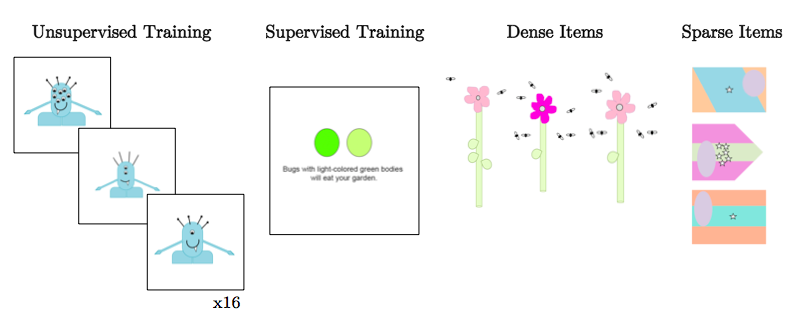
\includegraphics[width=\textwidth]{manipulations}
\caption[Example stimuli for category learning task]{Examples of learning type and category type manipulations for category learning experiment.}
\vspace{-10pt}
\label{sloutskymanip}
\end{figure}
	This task is within-subjects. Based on the group they were placed into, participants completed two of the four possible learning-category type combinations. In this experiment, I tested three main order effects. First, I tested order effects for the matching conditions (unsupervised-dense and supervised-sparse).The second order effect used unsupervised-dense and supervised-dense blocks. Finally, the third order effect tested the same sparse stimuli, testing unsupervised-dense and supervised-sparse blocks. This design led to six possible order groups that each participant could be placed into. See Table \ref{exp1order} for a summary. 

\begin{wraptable}[11]{r}{0.6\linewidth}
\caption{Block orders for statistical density task}
%\vspace{-10pt}
\begin{center}
\begin{tabular}{ c|c|c|c } 
 \hline 
 Effect & Group & Block 1 & Block 2 \\ 
 \hline
 \multirow{2}{*}{1} & 1 & Unsupervised-dense & Supervised-sparse \\ 
 & 2 & Supervised-sparse & Unsupervised-dense \\ 
 \hline
  \multirow{2}{*}{2} & 3 & Unsupervised-dense & Supervised-dense \\ 
 & 4 & Supervised-dense & Unsupervised-dense \\
 \hline 
  \multirow{2}{*}{3} & 5 & Unsupervised-sparse & Supervised-sparse \\ 
 & 6 & Supervised-sparse & Unsupervised-sparse \\ 
 \hline
\end{tabular}
\end{center}
\vspace{-20pt}
\label{exp1order}
\end{wraptable} \par
 In each block, participants were introduced to the task through a short cover story. They were told to learn which items go with a certain property (e.g., which aliens are friendly). Crucially, no labels were attached to the categories (e.g., some aliens are Ziblets). Then, participants completed a training block (either supervised or unsupervised). After training, participants completed 40 test trials (16 target, 16 distractor, 8 catch), following the design of \citet{Kloos2008} . In each trial, participants saw a single item and used the keyboard to indicate whether the item matched the category they had just learned (e.g., if the alien is friendly). Catch items looked significantly different than both the target and competing categories, so participants should have always rejected them as members of the learned category. This experiment was presented using PsychoPy v.1.84.2 \citep{Peirce2007}. \par

\subsubsection{Behavioral Measures}
	I used multiple assessments to test participants' language ability.  The choice of assessments was based on the epiSLI criteria for language impairment \citep{Tomblin1996}, which includes comprehension, expression, vocabulary, grammar, and narrative. I adapted these requirements from a kindergarten population to a college-aged population. The epiSLI criteria have been shown to be robust for diagnosis of specific language impairment (SLI). In addition, other studies of language impairment more broadly have adapted a similar multidimensional approach to measuring language ability, sometimes including measures of phonological skills \citep{Catts2006}. Thus, using assessments that the many domains of language outlined in epiSLI criteria will allow me to get a fuller picture of individual differences in language ability. See Table \ref{slitable} for a summary of the assessments and which domains of the epiSLI criteria they cover. The specific tests used in this experiment are detailed below. \par
	\textbf{Test of word reading efficiency (TOWRE) phonemic decoding subtest.} TOWRE is a test of nonword fluency \citep{Torgesen1992}. This test is a part of the comprehension aspect of epiSLI, since the comprehension measure is reading-based. In the TOWRE, individuals have 45 seconds to read as many nonwords as possible. The nonwords become longer and more difficult as the list goes on. The raw score from the TOWRE is calculated by counting the number of words correctly pronounced before the time limit. These raw scores are then converted to standard scores using age-based norms. The standard scores are based on a distribution with a mean of 100 and a standard deviation of 15. In the current age range, a perfect raw score (63) on the TOWRE returns a standard score of "\textgreater 120." For the purposes of this study, scores of "\textgreater 120" will be trimmed to simply 120. \par
	\textbf{Woodcock Johnson-III word attack (WA) subtest.} This task measures nonword decoding ability \citep{Woodcock2001}. Like the TOWRE, it is helpful for measuring the comprehension aspect of epiSLI. However, while the TOWRE measures word fluency, this task measures decoding accuracy. Participants read a list of nonwords out loud at their own pace. Raw scores are calculated by counting the number of words the participant said correctly. Raw scores are converted to standard scores using age-based norms. The standard score distribution has a mean of 100 and a standard deviation of 15. \par
	\textbf{Computerized reading comprehension.} This test covers the comprehension and narrative aspects of epiSLI. This computerized reading comprehension (CRC) test is based on the Kaufman Test of Educational Achievement (KTEA) reading comprehension subtest \citep{Kaufman2004}. To create this test, I copied the passages and questions contained in the KTEA reading comprehension subtest into E-Prime \citep{schneider2002prime} for presentation on a computer. Then, I created multiple choice answers for the KTEA questions that did not already have them. In this task, participants read short expository and narrative texts and answer multiple-choice comprehension questions about them. Some questions are literal, while others require participants to make an inference. Participants completed as many questions as they could in 10 minutes. Once 10 minutes had elapsed, the participant was allowed to answer the question currently on the screen and then the assessment closed. Because this task is a modified version of the KTEA, I use raw scores in analysis rather than standardized scores based on the KTEA norms. Raw scores are calculated by counting the number of correctly answered questions for each participant.  \par
	\textbf{Nelson-Denny vocabulary subtest.} The Nelson-Denny vocabulary sub-test is a written assessment of vocabulary \citep{Brown1981}. This test covers the vocabulary aspect of epiSLI. This test has been used in multiple studies of college-aged adults and provides sufficient variability for individual difference investigations in this population \citetext{e.g., \citealt{Boudewyn2015}; \citealt{Stafura2014}}. In this test, participants are asked to choose the word closest to a target vocabulary word. The test has a total of 80 items. Participants were allowed unlimited time to complete all items. Raw scores were generated by counting the total number of correctly answered items. The raw scores were then converted to standard scores based upon a norming sample including students in 10th, 11th, and 12th grade as well as two- and four-year college students. The standard scores for this assessment have a mean of 200 and a standard deviation of 25. \par
	\textbf{Clinical Evaluation of Language Fundamentals recalling sentences subtest.} I will use the recalling sentences subtest from the Clinical Evaluation of Language Fundamentals - Fourth Edition \citetext{CELF; \citealt{Semel2006}}. This test covers the grammar and expression aspects of epiSLI. In this subtest, participants hear sentences and are asked to repeat them. Scoring is based on how many errors the participant makes in their repetition. Raw scores are calculated by adding up the number of points achieved for each item. These are then converted to standard scores using age-based norms. The standard scores are based on a distribution with a mean of 10 and a standard deviation of 3. \par
	\textbf{Raven's Advanced Matrices.} Finally, I used Set II of Raven's Advanced Matrices (RAM) to measure nonverbal IQ \citep{Raven1998}. In this task, participants see a grid containing eight images and an empty space. The images are arranged in the grid according to some rule or rules. Participants must choose one of eight additional images that fits in the empty space. Due to time constraints, we restricted participants to 10 minutes in this task. Since this administration is different than the standard administration, we do not use standard scores. Raw scores are calculated by counting the number of correct answers given within 10 minutes.

\begin{table}[H]
\caption{Assessments of language and their corresponding epiSLI domains.}
\vspace{-10pt}
\begin{center}
\begin{tabular}{ c|c } 
 \hline 
 Test & epiSLI Criteria \\ 
 \hline
 TOWRE & \multirow{2}{*}{Comprehension (decoding aspect)}\\ 
 WA & \\ 
 CRC & Comprehension, narrative \\
 ND Vocab & Vocabulary \\ 
 CELF RS & Grammar, expression \\ 
 \hline
\end{tabular}
\end{center}
\label{slitable}
\end{table}


\subsection{Procedure}
	Each participant completed the category learning task as well as all of the behavioral measures. TOWRE, WA, and CELF were audio-recorded to allow for offline scoring. To allow multiple subjects to be run in a single timeslot, some participants received tasks they could complete on their own (category learning, ND, computerized reading comprehension, Raven's) first while others completed tasks with the experimenter first (WA, CELF, TOWRE). All together, the seven tasks took approximately one hour.
	
\subsection{Results}
	For all analyses shown below, accuracy was converted to \textit{d'} values \citep{macmillan2004} using the R package \textbf{neuropsychology} \citep{neuropsych}. Correction for extreme values was done following \citep{Hautus1995}. Following prior research, all blocks where 5 or fewer catch items were correctly rejected were dropped from analysis. This resulted in 22 total missing blocks (out of 458 total), including both blocks from a single subject in group 5. For basic descriptive statistics on the category learning task, see Table \ref{exp1expdesc}. For reaction time, all incorrect trials were dropped, as well as any trials with a response faster than 250ms.  \par

\begin{table}[H]
\caption{Descriptive statistics for the category learning task.}
\vspace{-10pt}
\begin{center}
\begin{tabular}{ccccc}
\hline
Order Effect       & Group              & Block               & Mean (SD) Accuracy & Mean (SD) RT (ms) \\ \hline
\multirow{4}{*}{1} & \multirow{2}{*}{1} & Unsupervised-dense  & 0.91 (0.19)        & 1074 (697)        \\ \cline{3-5} 
                   &                    & Supervised-sparse   & 0.93 (0.14)        & 809 (549)         \\ \cline{2-5} 
                   & \multirow{2}{*}{2} & Supervised-sparse   & 0.72 (0.34)        & 864 (608)         \\ \cline{3-5} 
                   &                    & Unsupervised-dense  & 0.90 (0.18)        & 834 (563)         \\ \hline
\multirow{4}{*}{2} & \multirow{2}{*}{3} & Unsupervised-dense  & 0.91 (0.18)        & 1063 (674)        \\ \cline{3-5} 
                   &                    & Supervised-dense    & 0.91 (0.23)        & 946 (636)         \\ \cline{2-5} 
                   & \multirow{2}{*}{4} & Supervised-dense    & 0.90 (0.21)        & 960 (679)         \\ \cline{3-5} 
                   &                    & Unsupervised-dense  & 0.92 (0.18)        & 861 (561)         \\ \hline
\multirow{4}{*}{3} & \multirow{2}{*}{5} & Unsupervised-sparse & 0.57 (0.35)        & 1275 (761)        \\ \cline{3-5} 
                   &                    & Supervised-sparse   & 0.93 (0.14)        & 812 (543)         \\ \cline{2-5} 
                   & \multirow{2}{*}{6} & Supervised-sparse   & 0.93 (0.12)        & 866 (592)         \\ \cline{3-5} 
                   &                    & Unsupervised-sparse & 0.53 (0.38)        & 1003 (633)        \\ \hline
\end{tabular}
\label{exp1expdesc}
\end{center}
\end{table}

\subsubsection{Behavioral Assessments}
\begin{wraptable}[14]{r}{0.6\linewidth}
\begin{center}
\caption{Descriptive Statistics for Behavioral Measures}
\begin{tabular}{L|c|c|c}
Assessment                         & Mean & SD   & Range   \\
\hline 
CELF Recalling Sentences SS        & 10.7 & 1.86 & 3-14    \\
Computerized Reading Comprehension & 21.7 & 5.12 & 7-48    \\
Nelson-Denny Vocabulary SS         & 229  & 14.0 & 175-255 \\
TOWRE SS                           & 96.2 & 9.86 & 59-120  \\
Word Attack SS                     & 99.7 & 9.04 & 75-120  \\
Raven's Advanced Matrices          & 15.1 & 4.58 & 0-26   
\end{tabular}
\label{exp1behdesc}
\end{center}
\end{wraptable}
\par
	For basic descriptive statistics on the behavioral measures, see Table \ref{exp1behdesc}. Before performing any statistical analyses using the individual difference measures, I checked their normality using the D'Agostino normality test from the R package \textbf{fBasics} \citep{fBasics}. Four measures (CRC, ND Vocab, CELF RS, RAM) were significantly skewed. These measures were centered, scaled, and transformed using Yeo-Johnson transformations from R package \textbf{caret} \citep{caret}. The remaining measures (TOWRE, WA) were not skewed and thus were simply scaled and centered. \par
	Since my goal was to create a composite measure of language ability, I investigated the relationship between the behavioral measures. First, I constructed a correlation matrix between all of the behavioral measures (see Table \ref{exp1behcorr}). All pairs of measures had a significant positve correlation with the exception of CELF RS and RAM. To further test whether the behavioral measures could be combined into a single composite, I ran a principal components analysis (PCA) on the 5 assessments related to epiSLI (i.e., all assessments except RAM). The Kaiser-Meyer-Olkin overall measure of sampling adequacy was 0.69, above the commonly accepted threshold of 0.6. Bartlett's test of sphericity was also significant $\chi^{2}(10)$  = 236.16, \textit{p} \textless 0.001. These suggest that the 5 behavioral assessments were suitable for a PCA. \par
	The first component in the PCA accounted for 47.74\% of the variance and had an eigenvalue of 2.38. All of the factor loadings for this component were quite similar, ranging from -0.41 to -0.51. The second factor accounted for an additional 20.5\% of the variance and had an eigenvalue of 1.02. This factor separated the two measures involved in decoding (TOWRE and WA) from the other measures (CRC, ND Vocab, and CELF RS). The remaining components had eigenvalues below 1. Thus, of the two significant components, the first component explained almost half of the variance and had an eigenvalue more than double the second component, which largely represented decoding ability. Since the first component indicated that most of the measures loaded similarly, I decided to take a simple means approach to creating a language composite measure. \par
	The language composite measure was created by averaging the 5 scaled, centered, and/or transformed measures. For participants with missing behavioral measures, the composite was created by averaging the remaining available measures. No subject was missing more than 1 measure. This composite measure was then scaled but not centered. This language composite measure and the centered, scaled, and transformed RAM measure are used in the analyses investigating order effects reported below.
	
\begin{table}[H]
\caption{Correlations between behavioral measures.}
\vspace{-10pt}
\begin{center}
\begin{tabular}{l|l|l|l|l|l|l}
                                      & 1       & 2       & 3       & 4      & 5       & 6 \\
1. Computerized Reading Comprehension & -       &         &         &        &         &   \\
2. Nelson-Denny Vocabulary            & 0.57*** & -       &         &        &         &   \\
3. CELF Recalling Sentences           & 0.31*** & 0.40*** & -       &        &         &   \\
4. Raven's Advanced Matrices          & 0.31*** & 0.34*** & 0.09    & -      &         &   \\
5. TOWRE                              & 0.22**  & 0.28*** & 0.26*** & 0.16*** & -       &   \\
6. Word Attack                        & 0.22**  & 0.38*** & 0.29*** & 0.22*** & 0.53*** & -
\end{tabular}
\label{exp1behcorr}
\end{center}
\vspace{-10pt}
\caption*{*\textit{p} \textless 0.05, **\textit{p} \textless 0.001, ***\textit{p} \textless 0.0001}
\end{table}

		
\subsubsection{Order Effect 1: Matching Conditions}
	The first analysis investigated order effects for blocks in which the learning type (supervised vs. unsupervised) and category type (sparse vs. dense) both engaged the same category learning system (hypothesis testing vs. associative). Participants completed supervised-sparse and unsupervised-dense blocks.  \par
	\textbf{Accuracy.} I used linear mixed-effects models to examine the effects of block and order on accuracy at test. Accuracy in these models was measured by \textit{d'} values for each subject by block. The base model included random intercepts for subject. Adding block and order as fixed effects significantly increased model fit, $\chi^{2}(2)$ = 13.21,  \textit{p} = 0.001. Adding the interaction between block and order further improved model fit, $\chi^{2}(1)$ = 6.03,  \textit{p} = 0.014. Thus, the final model including only experimental conditions had fixed effects of block, order, and the interaction between block and order as well as random intercepts for subject. \par
	This model revealed two significant effects. First, there was a significant main effect of order, \textit{F}(1,75) = 8.60, \textit{p} = 0.004. There was also a significant interaction between block and order, \textit{F}(1,74) = 6.10, \textit{p} = 0.02. There was not a significant main effect of block, \textit{F}(1,76) = 2.61, \textit{p} = 0.11. The interaction was broken down by conducting two separate models for each of the orders (unsupervised-dense first and supervised-sparse first). These analyses showed that when the associative system was engaged first (unsupervised-dense first), there was no significant main effect of block, \textit{F}(1,36) = 0.014, \textit{p} = 0.91. When the hypothesis testing system was used first (supervised-sparse first), there was a significant effect of block, \textit{F}(1,37) = 7.52, \textit{p} = 0.009. This shows that when participants complete engage the hypothesis-testing system first, performance on the supervised-sparse (hypothesis-testing) block is lower than in the unsupervised-dense (associative) block (see Table \ref {exp1expdesc} Figure \ref{oes}). \par
	To investigate the effect of individual differences in language ability on the order effect, I used the final model above which included main effects for block and order as well as their interaction. I then added  the language composite measure as a fixed effect. I also added RAM to control for nonverbal IQ. This model revealed no significant effects for RAM or the language composite; there remained a significant interaction between block and order. \par
	\textbf{Reaction time}. Again, I used linear-mixed effects models to look at the effects of block and order on reaction time at test. While the accuracy measure was at the block level, reaction time here is modeled at the item level. The base model included random intercepts for subject and for block nested within subject. Adding the fixed effects of block and order increased the model fit, $\chi^{2}(1)$ = 21,02,  \textit{p} \textless 0.001. Further, adding the interaction between block and order improved model fit, $\chi^{2}(1)$ = 29.6,  \textit{p} \textless 0.001. \par
	This model showed three significant effects. There was a significant main effect of block, \textit{F}(1,72) = 52.42, \textit{p} \textless 0.001. There was also a significant main effect of order, \textit{F}(1,77) = 4.67, \textit{p} = 0.03. Finally, there was a significant interaction between block and order, \textit{F}(1,72) = 35.0, \textit{p} \textless 0.001. To break down this interaction, I ran follow-up models for each of the two orders. This showed that when the associative system was engaged first (unsupervised-dense first), there was a significant main effect of block, \textit{F}(1,37) = 53.6, \textit{p} \textless 0.001. When the hypothesis testing system was used first (supervised-sparse first), there was no significant effect of block, \textit{F}(1,35) = 0.30, \textit{p} = 0.59. This result is the opposite of what was found in accuracy. When the associative system is engaged first, we see a difference in RT between blocks, but when the hypothesis-testing system in engaged first, there is no difference in RT. \par
	Similar to the accuracy analysis, I added RAM and language ability as fixed effects to the final model from above. Neither one had any effect on RT. The main effects and interactions from above stayed significant. \par 
	\textbf{Summary.} While the findings from accuracy and reaction time seem to be opposing, they may in fact tell the same story. Group 1 engaged the associative system first. This group showed similar accuracy for both blocks but slower reaction time in their first block (unsupervised-dense/associative). Group 2 engaged the hypothesis-testing system first. They showed similar reaction times for both blocks, but lower accuracy in their first block (supervised-sparse/hypothesis-testing). Thus, both groups showed reduced performance (reflected in either reaction time or accuracy) on their first block, regardless of which system it engaged, perhaps reflecting a general learning effect across the task as a whole. Importantly, this learning effect is not modulated by language ability.

\subsubsection{Order Effect 2: Dense Stimuli}
	The second order effect analysis compared groups 3 and 4. All participants learned only dense categories, with the order of learning types differing between groups. \par
	\textbf{Accuracy.} Again, I used linear-mixed effects models to investigate the effects of block and order on accuracy at test. The base model included random intercepts for subject. Adding the fixed effects to the model did not significantly improve fit $\chi^{2}(2)$ = 0.07,  \textit{p} = 0.97. Indeed, neither block, \textit{F}(1,145) = 0.053, \textit{p} = 0.82, nor order, \textit{F}(1,145) = 0.016, \textit{p} = 0.90, were significant predictors of accuracy. Thus, accuracy at test on dense categories was similar regardless of training type or block order.
	Next, I conducted the individual differences analysis. Since the goal of this investigation was to see whether the relationship between order and accuracy in each block changed as a function of language ability, I created a model with fixed effects for block, order, and language ability as well as RAM. The model showed no significant effects of any of the predictors. \par 
	\textbf{Reaction time.} I used the same linear mixed-effects model as above, with random intercepts for subject and for block nested within subject in the base model. Adding fixed effects of order and block did not significantly improve model fit, $\chi^{2}(2)$ = 2.54, \textit{p} = 0.28. Block, \textit{F}(1,72) = 0.05, \textit{p} = 0.83, and order, \textit{F}(1,77) = 2.49, \textit{p} = 0.12, did not have any effect on reaction time. Adding language ability and RAM to the model also did not improve fit, $\chi^{2}(2)$ = 2.46, \textit{p} = 0.12. These measures were not significant predictors of reaction time for dense stimuli.\par
	\textbf{Summary.} There were no significant effects of block, order, or language ability found for dense stimuli. This may suggest that learning dense stimuli engages a single system regardless of the instructions. Alternatively, it may be that learning dense stimuli is overall an easy task, evidenced by the high accuracy values seen in these blocks.
	
\subsubsection{Order Effect 3: Sparse Stimuli}
	The third order effect investigated differences in learning sparse categories based on learning type order, using data from groups 5 and 6. \par 
	\textbf{Accuracy.} I used the same type of linear mixed-effect models as the prior two order effects, with random intercepts for subject. Adding block and order significantly increased model fit, $\chi^{2}(2)$ = 57.5, \textit{p} \textless 0.001. However, adding the interaction between block and order did not increase model fit, $\chi^{2}(2)$ = 0.33, \textit{p} = 0.56. Thus, the final model included fixed effects for order and block but not their interaction. This model revealed a significant main effect of block, \textit{F}(1,67) = 75.69, \textit{p} \textless 0.0001, but no significant main effect of order, \textit{F}(1,67) = 0.0008, \textit{p} = 0.98. Participants showed significantly higher accuracy in supervised-sparse blocks than in unsupervised-sparse blocks (see Table \ref{exp1expdesc}). \par 
	As in the two previous analyses, I added RAM and language ability to the final model above. Adding the language composite improved model fit even after adding RAM, $\chi^{2}(2)$ = 5.34, \textit{p} = 0.02. However, adding the interactions between block and language and order and language did not improve model fit, $\chi^{2}(2)$ = 1.94, \textit{p} = 0.38. The final model, which included no interactions, showed the same main effect of block seen above as well as a significant main effect of language ability, \textit{F}(1,63) = 5.21, \textit{p} = 0.03. The effect of language ability was associated with a positive coefficient, \textit{b} = 0.19, suggesting that accuracy and language ability were positively related. There was no main effect of RAM. \par 
	\textbf{Reaction time.} As above, I used a linear mixed-effect model with random intercepts for subject and block nested within subject as the base model. Adding the fixed effects of order and block significantly improved fit, $\chi^{2}(2)$ = 50.0, \textit{p} \textless 0.0001. In addition, adding the interaction between block and order improved fit,  $\chi^{2}(2)$ = 25.4, \textit{p} \textless 0.0001. The final model showed significant main effects for block, \textit{F}(1,67) = 39.46, \textit{p} \textless 0.0001, order, \textit{F}(1,70) = 4.56, \textit{p} = 0.04, as well as a significant interaction between block and order, \textit{F}(1,67) = 29.57, \textit{p} \textless 0.0001. Follow-up models showed that for each order, there was a significant difference in reaction time by block. However, the difference between mean reaction time of the two blocks for group 5 (unsupervised-sparse first) was 463 ms, while the difference for group 6 (supervised-sparse first) was 137 ms. This suggests that the interaction represents a greater difference between blocks for participants who received the unsupervised-sparse block first.  \par 
	For the individual differences analysis, I added RAM and the language composite to the final model from above. Adding the language composite did not improve the model fit. There was no effect of language ability on reaction time for sparse stimuli. \par
	\textbf{Summary.} In terms of accuracy, participants showed higher accuracy on the supervised-sparse block than on the unsupervised-sparse block, regardless of order. In addition, accuracy on all blocks was positively related to language ability. This relationship did not vary by block or order. For reaction time, we saw and interaction between block and order, but no effect of language ability. The unsupervised-sparse block was by far the most difficult block for all participants who received it. Thus, this interaction may reflect this block difference crossed with learning effects. Participants who received the unsupervised-sparse block second were perhaps more comfortable with the task overall than participants who received the unsupervised-sparse block first, which lead to shorter reaction times for those receiving unsupervised-sparse second.
	
\begin{figure}[H]
\vspace{-10pt}
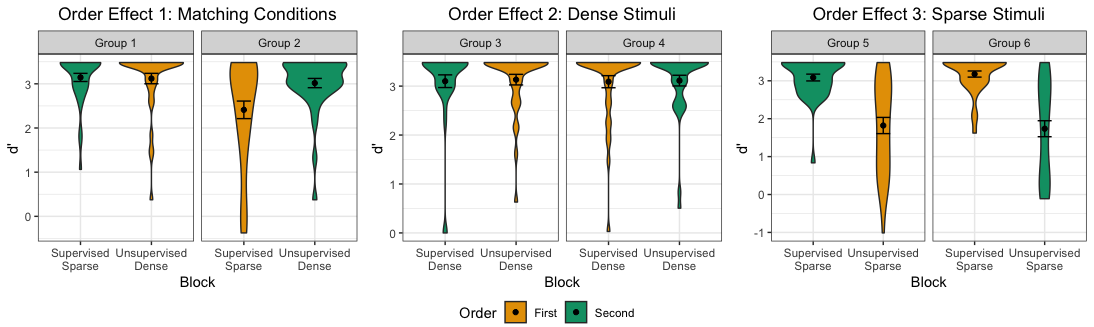
\includegraphics[width=\textwidth]{exp1_ordereffects.png}
\caption[Accuracy plot for all order effects]{Accuracy (d') for each block completed by each group for all order effects. Colors indicate which block was encountered first by each group. Points indicate means with error bars reflecting standard error. Shaded portions represent the distribution of accuracy values; wider portions indicate more subjects with that accuracy value.}
\label{oes}
\vspace{-10pt}
\end{figure}	

\begin{figure}[H]
\vspace{-10pt}
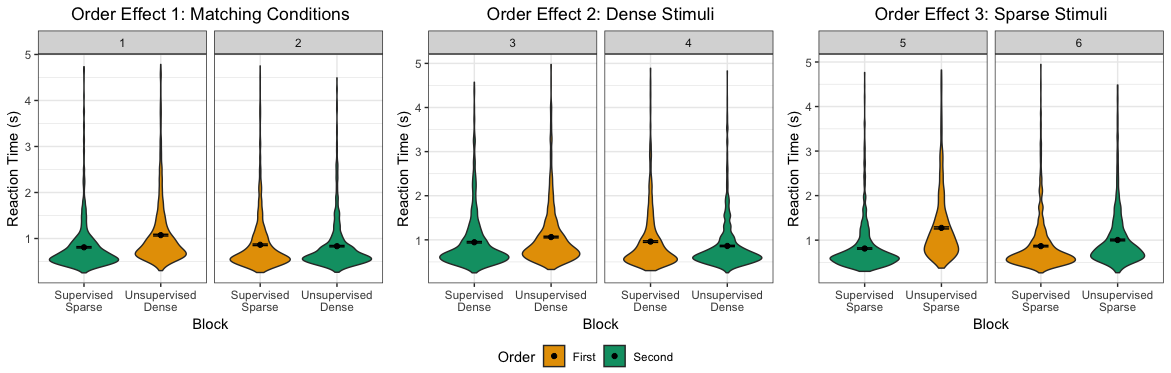
\includegraphics[width=\textwidth]{order_rt.png}
\caption[Reaction time plot for all order effects]{Reaction time (s) for each block completed by each group for all order effects. Colors indicate which block was encountered first by each group. Points indicate means with error bars reflecting standard error. Shaded portions represent the distribution of reaction times; wider portions indicate more trials with that reaction time.}
\label{oe_rt}
\vspace{-10pt}
\end{figure}	
	
\subsection{Discussion}
\subsubsection{Order Effects}
	
\subsubsection{Individual Differences}
\end{document}

